\section{Cơ sở lý thuyết}
\subsection{Thiết kế màn chơi}
\hspace*{1cm} Một màn chơi là không gian những gì cốt lõi diễn ra trong game. Nơi này đặt ra những giới hạn cho người chơi trong việc tương tác với game. Có sự đa dạng trong từng level. Mỗi level có thể có một số điểm tương đồng, nhưng mỗi màn sẽ có những nét đặc trưng khác nhau.\\
\hspace*{1cm} Thiết kế màn chơi là một giai đoạn của quá trình phát triển trò chơi nơi các nhà phát triển tập trung tạo ra các không gian này, bao gồm các cấp độ, bản đồ và nhiệm vụ trong game. Việc thiết kế trò chơi là việc kết hợp các yếu tố cấu thành nên trải nghiệm người chơi, bao gồm cơ chế game, gameplay, cốt truyện,...\\
\hspace*{1cm} Tuy nhiên, việc thiết kế màn chơi không phải để cho có. Việc thiết kế màn chơi cần có một mục đích nào đó, ví dụ như kể chuyện, có nhân vật và phục vụ cho mục đích rõ ràng trong game. Hơn hết, người thiết kế phải tập trung vào trải nghiệm người chơi, hơn là cảm nhận bản thân. Và màn chơi phải thực sự cuốn hút và vui để mang đến trải nghiệm cho người chơi\\
\hspace*{1cm} Mục tiêu của việc thiết kế màn chơi là tạo ra các sự kiện tương tác trong môi trường game sao cho chúng mang tính thử thách người chơi. Giúp người chơi đạt được cảm giác vui sướng khi hoàn thành và có mong muốn tiếp tục gắn bó với game.\\
\subsubsection{Các bước thiết kế một màn chơi}
\hspace*{1cm} Để thiết kế màn chơi, cần tập trung vào các bước chính sau:
\begin{enumerate}
	\item \textbf{Xác định lại giới hạn dự án}\\
	Các ý tưởng có thể có rất nhiều, trông chúng có thể rất hay nhưng mà ta cũng nên nhìn lại xem giới hạn của dự án có phù hợp cho ý tưởng này không, từ đó chọn được các ý tưởng phù hợp. Nó có thể đến từ bản chất của dự án hoặc kỹ thuật. Người thiết kế màn chơi cần hiểu rõ các giới hạn này để thiết kế màn chơi sao cho hợp lý.\\
	\hspace*{1cm} Về bản chất của dự án. Điều cần phải chú ý nhất là người chơi cũng như nền tảng hiện thực. Ta cần xác định đối tượng người chơi chủ đạo của game (là trẻ em, người trưởng thành hay người cao tuổi, là nam hay nữ, có phải là mẹ bỉm sữa hay không,...) cũng như nền tảng để chơi (mobile, PC hay console). Điều này ảnh hưởng đến thời gian hoàn thiện, độ dài và độ khó của màn chơi cũng như phong cách đồ hoạ. Những dự án làm trên mobile sẽ nhanh hơn so với PC hay console. Những trò chơi nhắm đến đối tượng trẻ em thì độ dài màn chơi sẽ ngắn, độ khó cũng dễ hơn cũng như phong cách đồ hoạ cũng sẽ nhẹ đô hơn so với các game dành cho lứa tuổi người trưởng thành. Ta không thể sản xuất một tựa game có phong cách đồ hoạ máu me, hoặc chủ đề có liên quan đến chiến tranh cho đối tượng là trẻ em được.\\
	\hspace*{1cm} Về vấn đề kỹ thuật, người thiết kế màn chơi phải giữ cho game có tính nhất quán về mặt công nghệ. Người thiết kế cần biết dự án sẽ sử dụng công nghệ nào, phong cách đồ hoạ ra sao, âm thanh, nhạc nền như thế nào. Một trò chơi không thể sử dụng lẫn lộn đồ hoạ pixel và đồ hoạ vector nếu không có mục đích cụ thể, hoặc có mục đích nhưng sử dụng không hợp lý. Một trò chơi về chiến tranh thế giới thời hiện đại không thể xuất hiện các yếu tố như pháp sư, phù thuỷ hay kiếm sĩ trong các tựa game RPG được. Ngược lại, một trò chơi RPG Fantasy nếu không có yếu tố liên quan đến thế giới thực thì không thể nào có thứ gọi là súng được. Ngoài ra  Ngoài ra, hiệu ứng ánh sáng và môi trường trong game cũng là một vấn đề đáng lưu tâm. Ở các tựa game kinh dị hù doạ hoặc truy đuổi, môi trường và ánh sáng sẽ tác động nhiều đến cảm xúc của người chơi, có thể tạo cho người chơi cảm giác hồi hộp, thót tim nếu sử dụng hợp lý.\\
	\hspace*{1cm} Dưới đây là một game có thiết kế màn chơi có vấn đè về kỹ thuật, trong việc sử dụng cả pixel art, vector art và hiệu ứng ánh sáng chưa hợp lý.\\
	\begin{figure}[H]
		\centering
		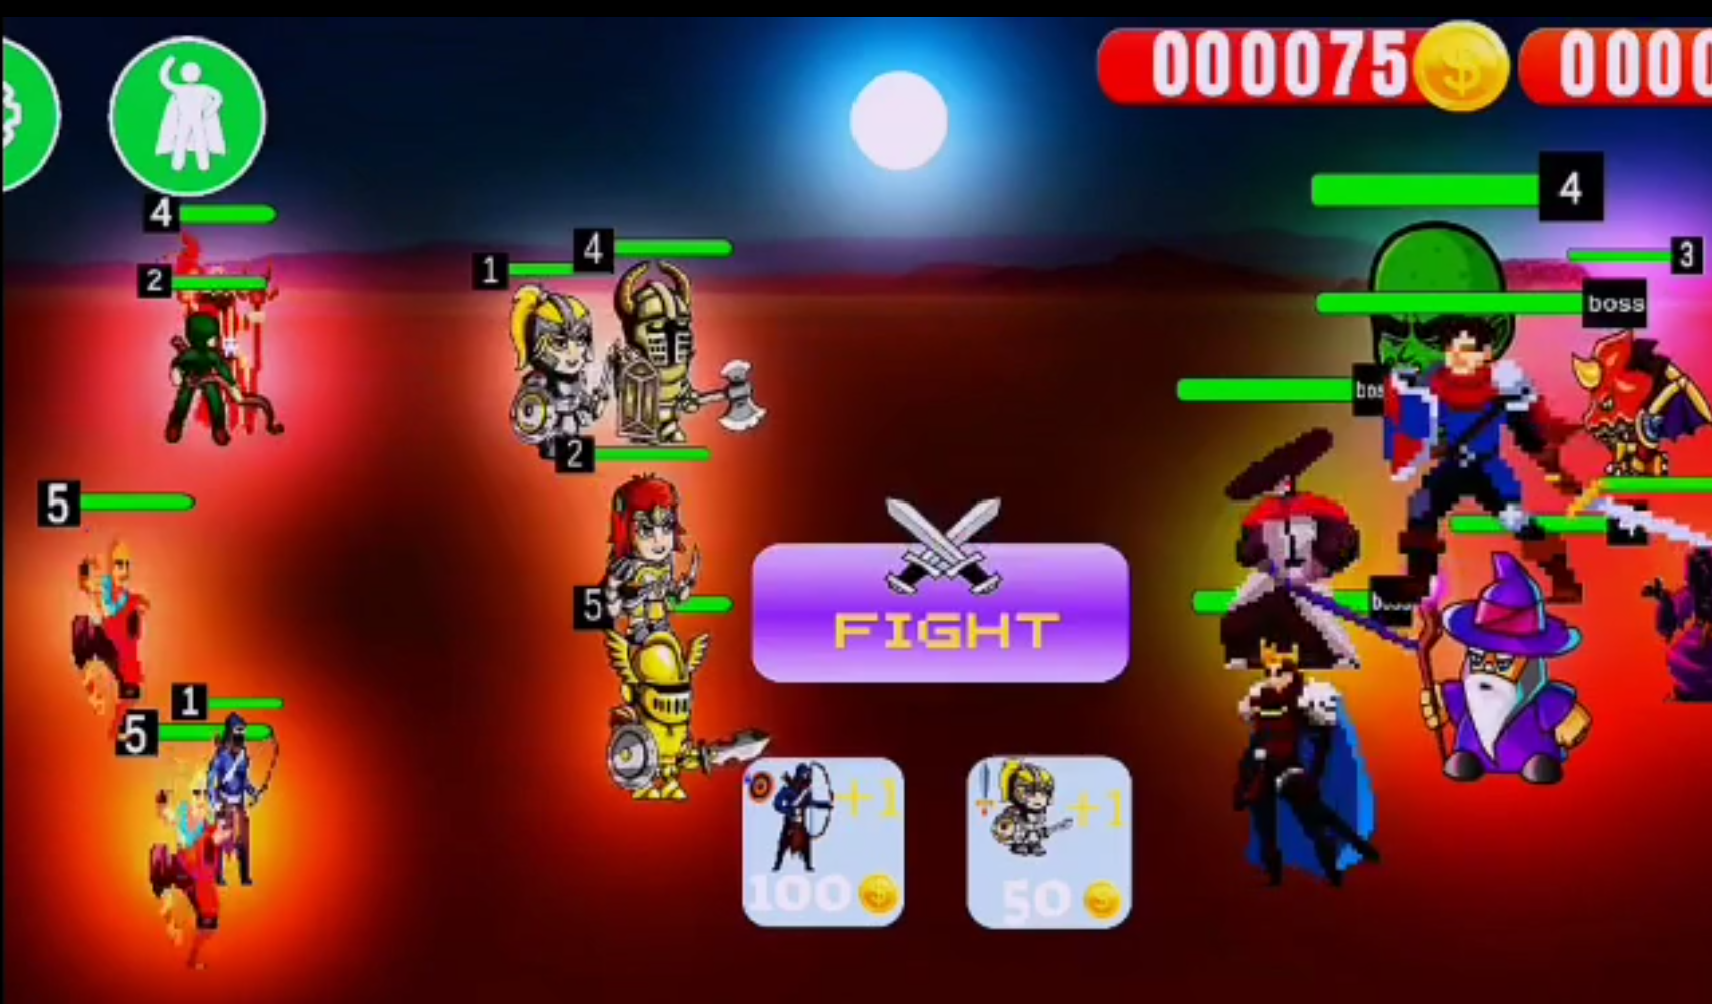
\includegraphics[width=\textwidth]{Images/AGameSuck.png}
		\vspace{0.5cm}
		\caption{Một màn chơi của game gặp vấn đề về kỹ thuật}
	\end{figure}

	\item \textbf{Lên ý tưởng và phác hoạ sơ bộ cấu trúc.}\\
	\hspace*{1cm}  Ở giai đoạn này, các thành viên khác trong dự án sẽ tiến hành lên ý tưởng và phác hoạ lên diẽn biến chính của cốt truyện cũng như xác định sơ bộ các thành phần khác của trò chơi như hình ảnh, âm thanh. Để việc thiết kế được dễ dàng hơn, người thiết kế có thể chia màn chơi thành các zone nhỏ sao cho dễ quản lý. Người thiết kế nên nghĩ đến màn chơi nếu chia thành nhiều zone sẽ ra sao và thiết kế từng zone riêng biệt để đạt hiệu suất cao và đơn giản hơn so với thiết kế toàn bộ màn chơi là một khối lớn.\\ 
	
	
	\item \textbf{Vẽ Bubble Diagram (lưu đồ Bong bóng).}\\
	\hspace*{1cm}  Trước khi bắt đầu đầu tư vào dự án, cần phải biết được tổng quan của các màn chơi sẽ như thế nào. việc giải thích bằng văn nếu không có sự hiệu quả sẽ gây khó hiểu cho người tiếp cận. Vì thế nên việc sử dụng lưu đồ sẽ phát huy tính hiệu quả, giúp cho người tiếp cận có cái nhìn tổng quan về màn chơi, bao gồm các zone chứa những gì và các zone được liên kết như thế nào. Ở giai đoạn này, sau khi phân chia màn chơi thành các vùng nhỏ và thiết kế chúng, người thiết kế sẽ kết nối các vùng đó với nhau thông qua một lưu đồ bong bóng.\\
	\textbf{Một số quy tắc khi vẽ lưu đồ:}
	\begin{itemize}
		\item Mỗi node trong đồ thị sẽ tượng trưng cho một zone của màn chơi.
		\item Mỗi node có thể kết nối với node khác bằng một và chỉ một mũi tên, đi từ ra từ node này đến node được chỉ định, một node có thể có thể có nhiều mũi tên chỉ ra, cũng như cũng có thể được nhiều mũi tên chỉ vào.
		\item Trên  mỗi mũi tên có thể có một ghi chú, có thể là điều kiện, ghi chú đường tắt,...
	\end{itemize}
	\begin{figure}[H]
		\centering
		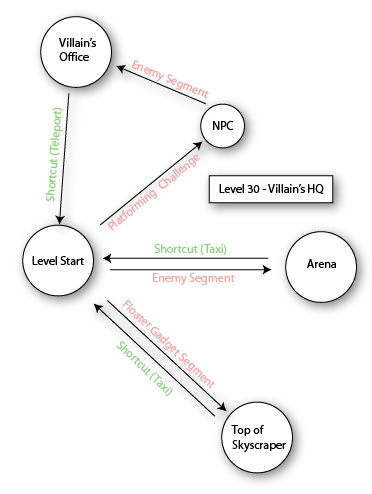
\includegraphics[width=7cm]{Images/bubblediagram.jpg}
		\vspace{0.5cm}
		\caption{Lưu đồ bong bóng}
	\end{figure}
	\hspace*{1cm} 
\end{enumerate}

% \subsection{Công nghệ}